% !TeX spellcheck = ru_RU
% !TEX root = vkr.tex

\section*{Введение}
% Использование линейной алгебры встречается в различных областях: от машинного обучения [ссылочка на статью] до теории графов [ссылочка на статью].
% \begin{enumerate}
%     \item Откуда и почему появляются разряженные матрицы.
%     \item Почему хочется улучшать производительность.
%     \item Почему выбран для этих целей template haskell.
%     \item Что такое kernel fusion.
%     \item Про template haskell
% \end{enumerate}
При работе с большими объёмами данных возникает множество проблем, одна из них~--- промежуточные структуры данных, которые никак не используются в результате, могут давать большую нагрузку на память и замедлять работу программы. Более или менее частные решения этой проблемы существуют: \textit{stream fusion}, дефорестация, суперкомпиляция, дистилляция.

Данные подходы имеют смысл, однако некоторые из них применимы только в крайне специфических областях, например, \textit{Tensorflow} для работы с тензорами, которые нужны для алгоритмов машинного обучения, или наоборот, крайне общие, очень теоретизированные и плохо \enquote{реально} изученные, например, дистилляция.

Таким образом, возникает идея изучения какого-то из наиболее общих методов в каких-то частных случаях для более лёгкого анализа.Слияние ядер~--- один из таких методов, он позволяет уменьшить количество промежуточных структур данных по средствам одновременной обработки узлов. Так как большинство литературы о новейших из этих методов используют модельные языки, имеющие функциональную природу, было решено писать на языке \Haskell{}, а в качестве частного случая рассматривать матрицы, представленные в виде деревьев квадрантов, крайне удобные для обработки в данной парадигме.
% 
\begin{figure}[h!]
    \centering
    \resizebox{0.45\textwidth}{!}{
        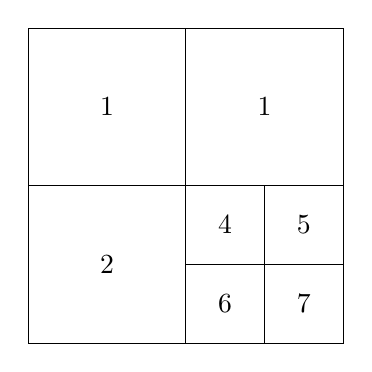
\begin{tikzpicture}
            \draw (1, 1) rectangle (3, 3);
            \node at (2, 2){2};
            \draw (1,3) rectangle (3, 5);
            \node at (2, 4) {1};
            \draw (3, 3) rectangle (5, 5);
            \node at (4, 4) {1};
            \draw (3, 1) rectangle (4, 2);
            \node at (3.5, 1.5) {6};
            \draw (3, 2) rectangle (4, 3);
            \node at (3.5, 2.5) {4};
            \draw (4, 1) rectangle (5, 2);
            \node at (4.5, 1.5) {7};
            \draw (4, 2) rectangle (5, 3);
            \node at (4.5, 2.5) {5};
        \end{tikzpicture}
    }
    \caption{Квадратная матрица, разделенная на квадранты}
    \label{qmatrix}
\end{figure}
\begin{figure}[h!]
    \centering
    \Tree [.A
            [.{Leaf(1, 2)}  ]
            [.{Leaf(1, 2)}  ]
            [.{Leaf(2, 2)}  ]
            [.SE
                    [.{Leaf(4, 1)}  ]
                    [.{Leaf(5, 1)}  ]
                    [.{Leaf(6, 1)}  ]
                    [.{Leaf(7, 1)}  ]
            ]
        !\qsetw{0.5cm}
    ]
    \caption{Изображение дерева квадрантов в виде дерева}
    \label{qtree1}
\end{figure}

